% Atwood Machines in TikZ (+Spring)
% Latexdraw.com
% 25/04/2020, 21:45

\documentclass[border=2mm]{standalone}
\usepackage{tikz}
\usetikzlibrary{decorations.pathmorphing,patterns}

\begin{document}

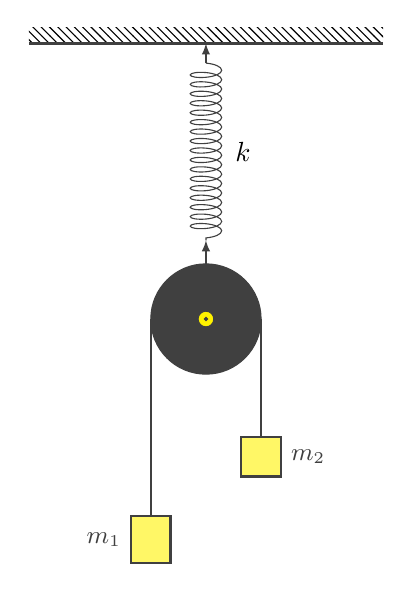
\begin{tikzpicture}[black!75]
% Supporting structure
\fill [pattern = north west lines] (-2.25,0) rectangle ++(4.5,.2);
\draw[thick] (-2.25,0) -- ++(4.5,0);

% Spring + Arrows
\draw[latex-] (0,0) -- ++(0,-0.25);
\draw[decoration={aspect=0.3, segment length=1.2mm, amplitude=2mm,coil},decorate] (0,-0.25) -- ++(0,-2.25) node[midway,right=0.25cm,black]{$k$}; 
\draw[latex-] (0,-2.5) -- ++(0,-0.3);


% Pulley
\draw[fill=black!75] (0,-3.5) circle(0.7cm);
\draw[fill=yellow] (0,-3.5) circle(0.1cm);
\draw[fill=black!75] (0,-3.5) circle(0.02cm);

% Mass 1
\draw[thick,fill=yellow!60] (-0.7,-3.5) -- ++(0,-2.5)
++(-0.25,-0.6) rectangle ++(0.5,0.6)
node[midway, left=0.25cm]{\small $m_1$} ;

% Mass 2
\draw[thick,fill=yellow!60] (0.7,-3.5) -- ++(0,-1.5)
++(-0.25,-0.5) rectangle ++(0.5,0.5)
node[midway, right=0.25cm]{\small $m_2$} ;

\end{tikzpicture}

\end{document}